\chapter{unused explosions}
\label{sec:cursor_crossed_a_line}
\lhead[tempest]{}
\lstset{style=6502Style}

The \textit{Tempest} source in \icode{ALSOUN.MAC} contains a couple of unused sound definitions.
The comment next to them suggests that they were originally intended as explosion effects.
\begin{lstlisting}
;
;EXPLOSION SOUND
;
T51F:   .BYTE 0C0,8,4,10
        .BYTE 0,0
T51A:   .BYTE 0A6,20,0F8,4
        .BYTE 0,0
T52F:   .BYTE 40,8,4,10
        .BYTE 0,0
T52A:   .BYTE 0A6,20,0FE,4
        .BYTE 0,0
\end{lstlisting}

When you listen to them they do sound like that alright. Give them a try below.

\begin{figure}[H]
{
    \begin{subfigure}{0.43\textwidth}
      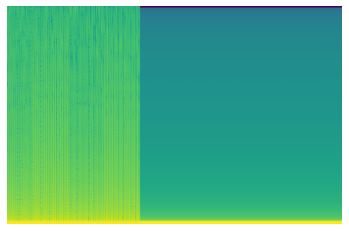
\includegraphics[width=6cm]{tempest_sounds/buttons/UNUSE1.raw-button.png}%
      \makebox[0pt][r]{%
        \raisebox{.6cm}{%
          \textattachfile{src/tempest_sounds/wav/UNUSE1.raw.wav}{
\includegraphics[width=3cm]{sounds/play.png}}%
        }\hspace*{1.50cm}%
      }%
      \caption*{T51F}
    \end{subfigure}
    \hspace{0.4cm}
    \begin{subfigure}{0.53\textwidth}
      
\includegraphics[width=6cm]{tempest_sounds/buttons/UNUSE2.raw-button.png}%
      \makebox[0pt][r]{%
        \raisebox{.6cm}{%
          \textattachfile{src/tempest_sounds/wav/UNUSE2.raw.wav}{
\includegraphics[width=3cm]{sounds/play.png}}%
        }\hspace*{1.50cm}%
      }%
      \caption*{T52F}
    \end{subfigure}
  }\caption*{The unused explosion sounds in \icode{ALSOUN.MAC}.}
\end{figure}
